\documentclass[article,nojss]{jss}
\DeclareGraphicsExtensions{.pdf,.eps}
\newcommand{\fct}[1]{{\code{#1()}}}
\newcommand{\class}[1]{{`\code{#1}'}}


\author{ Marco Smolla \And Bart Kranstauber}
\Plainauthor{Marco Smolla, Bart Kranstauber}

\title{Using the move package}
\Plaintitle{Using the move package}

\Keywords{animal track, time series, utilization density, gps}

\Abstract{
  This vignette gives examples of how to use the \pkg{move} package. It explains how to load data in the \pkg{move} functions using \fct{read.csv} and \fct{move}, transform data into a different projection method with \fct{spTransform}, and calculate the utilization density using \fct{brownian.bridge.dyn}. Further functions to extract information from the Move object and plot the track and utilization density will be explained as well. \\
}

\Address{
  Marco Smolla\\
  Max-Planck-Institute for Ornithology, Radolfzell, Germany\\
  E-mail: \email{msmolla@orn.mpg.de}\\

  Bart Kranstauber\\
  Max-Planck-Institute for Ornithology, Radolfzell, Germany\\
  E-mail: \email{kranstauber@orn.mpg.de}\\
}

\usepackage{Sweave}
\begin{document}



%\VignetteIndexEntry{How to use the move pacakge}
%\VignetteDepends{sp, raster, rgdal, methods, geosphere}
%\VignetteKeywords{GPS, time series, track}
%\VignettePackage{move}


\section*{Introduction}
The first set of functions the move package includes lets you import, analyse and visualize tracking data. A possible workflow could look like this: \\ \\
1. import data \\
2. transform coordinates to correct aeqd (Azimuthal Equidistant) projection \\
3. calculate utilization densities using the dynamic Brownian Bridge Movement Model\\
4. plot the track and the utilization density\\



%%%%%%%%%%%%%%%%%%%%%%%%%%%%%%%%%%%%%%%%%%%%%%%%%%%%%%%
\section*{Importing data}
\subsection*{Movebank data}
There are two ways to import data into the \pkg{move} functions. The easiest way is to work with downloaded files from \url{movebank.org}. With the following function you just have to define the path to the file like \texttt{move(x="path")}.

\begin{Schunk}
\begin{Sinput}
> data <- move(system.file("extdata","leroy.csv",package="move"))
\end{Sinput}
\end{Schunk}

\textbf{NOTE:} The command to load the example data set \texttt{leroy.csv} works only for this file, because it is part of the package. To import own data consider the help page of the \fct{move} function.

\subsection*{Non-Movebank data}
If you want to use data that are not from movebank, you can use the \fct{move} function as well. In this case you first need to import the \class{data.frame} with the ordinary \fct{read.table}. Afterwards you define which columns store the x and y coordinates and the timestamps. You also need to define the format of the timestamps and projection. The projection method must be a \class{CRS} and the timestamps a \class{POSIXct} object.

\begin{Schunk}
\begin{Sinput}
> file <- read.table(system.file("extdata","leroy.csv",package="move"), 
+           header=TRUE, sep=",", dec=".")
> data <- move(x=file$location.long, y=file$location.lat, 
+           time=as.POSIXct(file$timestamp, format="%Y-%m-%d %H:%M:%S", tz="UTC"), 
+           data=file, proj=CRS("+proj=longlat"))
\end{Sinput}
\end{Schunk}

In both cases you create an object of the class \class{Move}. It stores among others the timestamps and coordinates which are necessary for the following functions. 

%%%%%%%%%%%%%%%%%%%%%%%%%%%%%%%%%%%%%%%%%%%%%%%%%%%%%%%
\section*{Transform coordinates projection}
For technical reasons the coordinates of the Move object must be in the \texttt{aeqd}, or Azimuthal Equidistant, projection. To check the projection of your coordinates you can use the \fct{proj4string} method. If your data are not in the right projection, use the following command to change it. 

\begin{Schunk}
\begin{Sinput}
> proj4string(data)
\end{Sinput}
\begin{Soutput}
[1] " +proj=longlat +ellps=WGS84"
\end{Soutput}
\begin{Sinput}
> data2 <- spTransform(x=data, CRSobj="+proj=aeqd", center=TRUE)  
> proj4string(data2)
\end{Sinput}
\begin{Soutput}
[1] " +proj=aeqd +lon_0=-73.8871629 +lat_0=42.73884025 +ellps=WGS84"
\end{Soutput}
\end{Schunk}
The data are now in the right projection and the coordinate system is now centred to the center of the track. 

%%%%%%%%%%%%%%%%%%%%%%%%%%%%%%%%%%%%%%%%%%%%%%%%%%%%%%%
\section*{Using the dynamic Brownian Bridge Movement Model}
To calculate the utilization density (UD) with the dynamic Brownian Bridge Movement Model use the \fct{brownian.bridge.dyn} function. You need to specify the Move object from which you want to calculate the UD, the location error of your localization method (in map units), the raster options, and the extension of the raster. \\
You can either set the number of the raster cells along the longest dimension of your map by setting a numeric value for the \texttt{dimSize} argument, or - if you know the extent of your map - you can set the size of the raster cells with a numeric value for the \texttt{raster} argument (you can only set one of them). \\
When the \fct{brownian.bridge.dyn} function issues the warning, the extent of your raster is too small, that is that a large part of the UD is at the borders of the raster. You can change the extent of the raster by setting the \texttt{ext} argument. If you want to extend the raster in all four directions equally choose one number. Use a vector of two numbers to extend the x and the y dimension differently, or even a vector with four numbers to extend differently in all four directions. \\

\begin{Schunk}
\begin{Sinput}
> p <- brownian.bridge.dyn(object=data2, location.error=23.5, dimSize=45, ext=.3)
\end{Sinput}
\end{Schunk}

Running the \fct{brownian.bridge.dyn} creates an object of the \class{DBBMM} class, which among others stores the raster of the map with the values from the UD. 

%%%%%%%%%%%%%%%%%%%%%%%%%%%%%%%%%%%%%%%%%%%%%%%%%%%%%%%
\section*{Plotting data}
\subsection*{Plotting the track (Move object)}
To plot the track of the animal, simply use the following functions. You can just use \fct{plot} on a \class{Move} object and get the track with dots and lines. If you only want to plot points or lines use the respective functions. With the \texttt{add} and \texttt{col} arguments you can add the plots to another plot or change the colors. \\
If you want to plot the track of the animal on a real map, use the \fct{plot} function with the \texttt{google} argument set \texttt{TRUE}.\\
Figure 1 shows what the different functions create\footnote{With the \texttt{attach} and \texttt{par} command four plots are returned at once.}. 

\begin{Schunk}
\begin{Sinput}
> attach(mtcars)
> par(mfrow=c(2,2))
> plot(data2)
> points(data2, col="blue")
> lines(data2, col="green")
> plot(data, google=T)
\end{Sinput}
\end{Schunk}

\begin{figure}
\begin{center}
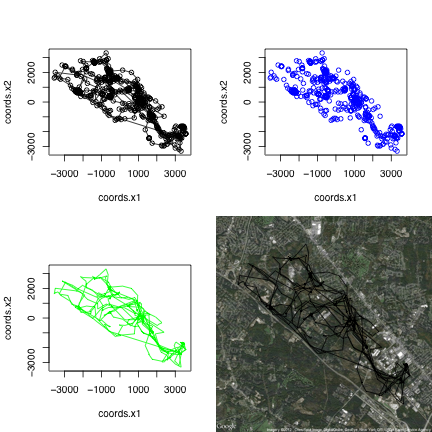
\includegraphics{move-fig1}
\end{center}
\caption{Different ways (lines, points, lines and points, google map) to display the track.}
\label{fig:one}
\end{figure}


%%%%%%%%%%%%%%%%%%%%%%%%%%%%%%%%%%%%%%%%%%%%%%%%%%%%%%%
\subsection*{Plotting the utilization density (DBBMM object)}
You might want to plot the \class{DBBMM} object you created earlier. Use the \fct{plot} function to produce a fixed cell size ratio graphic from the raster, or the \fct{image} function to produce a variable cell size ratio graphic (not prone to distortions after resizing the graphics window) from the raster. \\
To plot contour lines from the raster use the \fct{contour} function and set the percentage levels that you want to print. With \texttt{add=TRUE} you can add the contour to a previous plot. The same works if you want to add the track as lines or points, or both. \\
Figure 2 shows what this could look like. 


\begin{Schunk}
\begin{Sinput}
> attach(mtcars)
> par(mfrow=c(2,2))
> plot(p)
> image(p)
> plot(p)
> contour(p, levels=c(.5,.9), add=TRUE)
> image(p)
> lines(data2, add=TRUE, col="black")
\end{Sinput}
\end{Schunk}

\begin{figure}
\begin{center}
\includegraphics{move-fig2}
\end{center}
\caption{Different ways to display the utilization density (left \fct{plot}, right \fct{image}), including the \fct{contour} (left) and \fct{lines} (right) function.}
\label{fig:two}
\end{figure}


%%%%%%%%%%%%%%%%%%%%%%%%%%%%%%%%%%%%%%%%%%%%%%%%%%%%%%%
\newpage
\section*{Extract information}
The \class{Move} and the \class{DBBMM} object store a lot of data. There are a couple of functions you can use to easily extract them.


\subsection*{... from a Move object}
\fct{as.data.frame}     : extracts the spatial data frame\\
\fct{coordinates}       : extracts the coordinates of the Move object\\
\fct{n.locs}            : returns the number of tracked locations\\
\fct{proj4string}       : returns the projection of the coordinates\\
\fct{time.lag}          : calculates the time differences between coordinates (in minutes)\\

\subsection*{... from a DBBMM object}
\fct{raster}              : returns the information of the stored raster\\
\fct{outerProbability}    : calculates the probabilities of the UD at the border of the raster\\



\end{document}
